\chapter{Implementation Details} \label{ch:compilation}

This chapter introduces our concrete implementation of the CP compiler that
targets JavaScript. The full set of compilation rules can be found in
\autoref{sec:fiplus-js}. Our implementation is available in the supplementary
materials.

\section{From Elaboration Semantics to JavaScript Code Generation}

In the elaboration semantics presented in \autoref{ch:calculi}, we use a
$\lambda$-calculus with extensible records as the target. In the actual
compilation, records are modeled as JavaScript objects, and type indices are
realized as objects' property names. For example, $[[48,,true]]$ compiles to
\lstinline|{ int: 48, bool: true }| in JavaScript. Besides, record concatenation
can be directly represented by object merging using the spread syntax like
\lstinline|{ ...obj1, ...obj2 }|.

As we have mentioned, the formalized target language is a functional calculus,
but JavaScript is an imperative language. The mismatch in programming paradigms
is an important consideration when implementing the compilation to JavaScript.
We consider two designs of target forms: one is based on \emph{static single
assignment} (SSA)~\citep{cytron1991efficiently}, and the other is based on
\emph{destination-passing style} (DPS)~\citep{shaikhha2017destination}. We
eventually choose the latter due to performance reasons, which we will explain
next.

\begin{figure}
\centering
\begin{subfigure}{.37\textwidth}
\begin{lstlisting}[language=TypeScript]
const $1 = { int: 48 };
const $2 = { bool: true };
const $3 = { ...$1, ...$2 };
const $4 = { int: 32 };
const $5 = $chr.fun_char($4);
const $6 = { ...$3, ...$5 };
\end{lstlisting}
\caption{Before optimization: 6 objects.} \label{fig:six-objects}
\end{subfigure}%
\hspace{.1\textwidth}%
\begin{subfigure}{.33\textwidth}
\begin{lstlisting}[language=TypeScript]
const $1 = {};
$1.int = 48;
$1.bool = true;
const $2 = {};
$2.int = 32;
$chr.fun_char($2, $1);
\end{lstlisting}
\caption{After optimization: 2 objects.} \label{fig:two-objects}
\end{subfigure}
\caption{Simplified JavaScript code for $[[48 ,, true ,, chr 32]]$.}
\end{figure}

\paragraph{Reducing intermediate objects.}
In our initial design based on the SSA form, every subterm in a merge creates a
new object in the compiled JavaScript code. Consequently, there will be too many
intermediate objects that are useless. For example, consider the merge
$[[48 ,, true ,, chr 32]]$, where $[[chr]]$ is a function that converts an
integer to a character, and the compiled function has been stored in
\lstinline{$chr}. We need to create six JavaScript objects in the SSA-based
form, as shown in \autoref{fig:six-objects}. As mitigation, we adopt a new
design based on DPS. We just create one object for the merge (e.g.
\lstinline{$1} in \autoref{fig:two-objects}) and pass the variable down to
subterms to update their corresponding properties. To further prevent the
function application (e.g. $[[chr 32]]$) from creating any intermediate object,
we add an extra parameter when compiling all functions, including $[[chr]]$. The
destination object (e.g. \lstinline{$1}) is passed to the compiled function as
the last argument, and the function body will directly write to that argument
instead of creating a new object. In other words, \lstinline{$1} is an output
parameter while \lstinline{$2} is an input. As a result, we reduce the creation
of six objects to only two objects and avoid two object concatenations, as shown
in \autoref{fig:two-objects}.

\section{Parametric Polymorphism} \label{sec:poly}

\begin{figure}
\begin{subfigure}{\textwidth}
\begin{lstlisting}[language=TypeScript]
const $poly = {};
$poly['forall_fun_(1&int)'] = function ($A, $1) {
  $1['fun_' + toIndex([ ...$A, 'int' ])] = function ($x, $2) {
    for (const $A$elem of $A) $2[$A$elem] = $x[$A$elem];
    $2.int = 48;
  };
};
\end{lstlisting}
\caption{\lstinline{poly = /\\(A * Int). \\(x: A) -> x , 48}.} \label{fig:poly-def}
\end{subfigure}
\par\bigskip
\begin{subfigure}{\textwidth}
\begin{lstlisting}[language=TypeScript,deletekeywords=string]
const $3 = {};  const $4 = {};
$poly['forall_fun_(1&int)']([ 'string', 'bool' ], $4);
const $5 = {};  $5.string = 'foo';  $5.bool = true;
$4['fun_(bool&int&string)']($5, $3);
\end{lstlisting}
\caption{\lstinline{poly @(String & Bool) ("foo" , true)}.} \label{fig:poly-app}
\end{subfigure}
\par\bigskip
\begin{subfigure}{\textwidth}
\begin{lstlisting}[language=TypeScript]
function toIndex(tt) {
  const ts = tt.sort().filter((t, i) => t === 0 || t !== tt[i-1]);
  if (ts.length === 1) return ts[0];
  else return '(' + ts.join('&') + ')';
};
\end{lstlisting}
\caption{\lstinline{toIndex}: an auxiliary function for generating type indices at run time.} \label{fig:toIndex}
\end{subfigure}
\caption{Simplified JavaScript code for polymorphic terms.}
\end{figure}

\noindent
The compilation of polymorphic terms is not formalized in \autoref{ch:calculi},
so here we introduce our solution in more detail. The challenge posed by
parametric polymorphism is mainly because type arguments are unknown until type
application. For those terms whose types contain free variables, we can only
generate type indices at run time. For example, \autoref{fig:poly-def} shows the
simplified JavaScript code for the following definition in CP:
\begin{lstlisting}
poly = /\(A * Int). \(x: A) -> x , 48;
\end{lstlisting}
Here the notation \lstinline{/\(A * Int)} represents a type parameter
\lstinline{A} bound by a $\Lambda$-function where \lstinline{A} is disjoint with
\lstinline{Int}. The \lstinline{poly} function can be typed as
$\forall [[A*Int]].\, [[A -> A&Int]]$. We employ a \emph{de~Bruijn
index}~\citep{de1972lambda} to represent the bound variable \lstinline{A}, so
the $\Lambda$-function's type index is \lstinline{"forall_fun_(1&int)"}. In
contrast, the inner $\lambda$-function's type index is more intriguing. Before
we introduce our approach, let us first see an example of applying
\lstinline{poly}:
\begin{lstlisting}
poly @(String & Bool) ("foo" , true)
\end{lstlisting}
The type parameter is instantiated with an intersection type
(\lstinline{String & Bool}), and \autoref{fig:poly-app} shows the simplified
JavaScript code for the application. After \lstinline{poly} is instantiated, the
inner $\lambda$-function will be used with concrete type indices (e.g.
\lstinline{"fun_(bool&int&string)"}) instead of something like
\lstinline{"fun_(A&int)"}. To achieve this, we pass the instantiated type as an
argument to the outer $\Lambda$-function. The argument is in the form of a
JavaScript array, which consists of the component types in the case of an
intersection type. The array is empty for top-like types, or it is a singleton
array for non-intersection, non-top-like cases. We also predefine a
\lstinline{toIndex} function to help generate the type index based on the
runtime instantiation, whose definition is shown in \autoref{fig:toIndex}. The
\lstinline{toIndex} function accepts an array of types and generates their
intersection's type index. To fit in with the notion of equivalent types in
\autoref{sec:eqty}, it will sort and deduplicate the component types. Now that
some type indices are dynamically generated, we have to use
\lstinline{obj[toIndex($A)]} instead of \lstinline{obj.name} directly. Such a
feature is called first-class labels~\citep{leijen2004first} and is supported in
JavaScript via computed property names with brackets. The situation in
\autoref{fig:poly-def} is a bit more complicated because the type of the inner
$\lambda$-function is $[[A -> A&Int]]$, so the dynamically computed type index
is \lstinline{"fun_" + toIndex([ ...$A, "int" ])}.

As illustrated above, the compiled code for polymorphic definitions incurs
overhead due to the dynamic computation of type indices. In mainstream
languages, parametric polymorphism is implemented via either
\emph{erasure}~\citep{igarashi2001featherweight} or
\emph{monomorphization}~\citep{griesemer2020featherweight}. Our compilation
scheme cannot erase type information at run time, so monomorphization is a
potential direction for improving the performance of polymorphic code. We leave
this for future work.

\section{Lazy Evaluation}

\begin{figure}
\begin{subfigure}{.25\textwidth}
\begin{lstlisting}[language=TypeScript,showlines]
const $1 = {};
$1['rcd_x:int'] = $1['rcd_y:int'];

\end{lstlisting}
\caption{By value.} \label{fig:call-by-value}
\end{subfigure}
\begin{subfigure}{.34\textwidth}
\begin{lstlisting}[language=TypeScript]
const $1 = {};
$1.__defineGetter__(
  'rcd_x:int',
  function () {
    return $1['rcd_y:int'];
  });
\end{lstlisting}
\caption{By thunk.} \label{fig:call-by-name}
\end{subfigure}
\begin{subfigure}{.39\textwidth}
\begin{lstlisting}[language=TypeScript]
const $1 = {};
$1.__defineGetter__(
  'rcd_x:int',
  function () {
    delete this['rcd_x:int'];
    return this['rcd_x:int'] = $1['rcd_y:int'];
  });
\end{lstlisting}
\caption{By memoized thunk.} \label{fig:call-by-need}
\end{subfigure}
\caption{Simplified JavaScript code for \lstinline|\{ x = this.y \}|.}
\end{figure}

\noindent
In the most recent work by \citet{fan2022direct}, \fiplus is formalized as a
call-by-name calculus to correctly model trait instantiation. A simple example
is as follows:
\begin{lstlisting}
type Rcd = { x: Int; y: Int };
new (trait [this: Rcd] => { x = this.y; y = 48 })
\end{lstlisting}
The program will not terminate if evaluated using the call-by-value strategy.
That is why \citeauthor{fan2022direct} go for a call-by-name semantics and
evaluate record fields lazily. However, a naive call-by-name implementation may
evaluate the same record field more than once and cause a significant slowdown.
Even with proper memoization (call-by-need), the performance of generated code
is still not ideal as JavaScript does not support lazy evaluation natively. In
our implementation, we employ a hybrid strategy: only self-annotated trait
fields are lazily evaluated, and other language constructs including function
applications are strictly evaluated. This approximates the semantics in
conventional OOP languages, which are call-by-value in terms of initializing
fields and calling methods, except for lazy fields.

To better illustrate different evaluation strategies for record fields, we show
three code snippets generated for the field \lstinline|{ x = this.y }|.
\autoref{fig:call-by-value} employs strict evaluation, but instead of
non-termination, the issue here is that the field \lstinline{y} is not yet
available, so field \lstinline{x} is unexpectedly assigned
\lstinline{undefined}. This issue severely limits self-references, and the code
in \autoref{fig:call-by-value} would be broken. Thus we need a better approach.
\autoref{fig:call-by-name} resolves the issue by adding a \emph{thunk}. The
field is wrapped in a getter, and thus the computation of \lstinline{this.y} is
delayed until the whole record is constructed with the field \lstinline{y}
available. But note that the getter is called every time the field is accessed.
This is undesirable as the computation in the thunk would be triggered on every
access to the field. We optimize this by memoizing fields using \emph{smart
getters}\footnote{\url{https://developer.mozilla.org/en-US/docs/Web/JavaScript/Reference/Functions/get\#smart_self-overwriting_lazy_getters}}.
As shown in \autoref{fig:call-by-need}, once the field is evaluated, the getter
is deleted, and the value is stored instead. Our implementation automatically
detects self-annotated trait fields and applies the last approach to them; for
other cases, the first approach is applied. By this means, self-references and
trait instantiation in CP are correctly supported while maintaining good
performance for other language constructs.

\section{Important Optimizations}

\paragraph{Eliminating redundant coercions.} \label{sec:elim}
In the rules of coercive subtyping shown in \autoref{fig:source-subtype}, even
$A <: A$ may go through a lot of rules when $A$ is a complex intersection type.
However, as long as we encounter subtyping between \emph{equivalent} types, we
do not need any coercion code. To implement this optimization, an immediate idea
would be:
\begin{itemize}
\item Adding a special case to \rref{Ela-Sub} such that if $[[A ~~ B]]$ then $[[t1]] = [[t2]]$.
\end{itemize}
Unfortunately, this rule does not deal with many important cases. For instance,
when checking $[[A -> B]] <: [[A -> C]]$, we would like to avoid applying
coercions to the inputs of the function (since they have the same type).
Therefore, besides the rule above, we may consider:
\begin{itemize}
\item Adding an extra rule (say \textsc{S-Equiv} in \autoref{fig:coerce})
      such that if $[[A ~~ B]]$ then $[[t : A <: B ~~> t]]$.
\end{itemize}
However, this idea is incorrect when an intersection type occurs on the
left-hand side. For example, when upcasting $[[48 ,, true]]$ to type $[[Int]]$,
the coercion is missing in the subtyping derivation:
\begin{mathpar}
\inferrule*[right=S-AndL]
 {\inferrule*[right=S-Equiv]
  {[[Int ~~ Int]]}
  {[[{int|=>48;bool|=>true} : Int <: Int ~~> {int|=>48;bool|=>true}]]}}
 {[[{int|=>48;bool|=>true} : Int&Bool <: Int ~~> {int|=>48;bool|=>true}]]}
\end{mathpar}
Observing that \rref{S-AndL,S-AndR} are the root cause of missing coercions, we
add an extra flag that indicates the applicability of rule \textsc{S-Equiv} to
fix the latter idea. As shown in \autoref{fig:coerce}, by default ($<:^+$) the
optimization \textsc{S-Equiv} can apply, but it will be disabled ($<:^-$) in the
derivations of rule \textsc{S-AndL} (as well as rule \textsc{S-AndR}), and
re-enabled in derivations of rule \textsc{S-Arrow} (as well as rules
\textsc{S-All} and \textsc{S-Rcd}). In some rules, the flag does not matter, so
we use $<:^\pm$ to mean that both cases apply. The complete rules targeting
JavaScript can be found in \autoref{sec:fiplus-js}.

\begin{figure}
\begin{ottdefnblock}{$[[t1]]:[[A]]\ottsym{<:}^\pm[[B]][[~~>]][[t2]]$}{Optimized coercive subtyping}
  \inferrule[S-Equiv]
  {[[ A ~~ B ]]}
  {[[t]]:[[A]]\ottsym{<:}^+[[B]][[~~>]][[t]]}

  \inferrule[S-AndL]
  {[[t]]:[[A]]\ottsym{<:}^-[[C]][[~~>]][[t']]}
  {[[t]]:[[A&B]]\ottsym{<:}^\pm[[C]][[~~>]][[t']]}

  \inferrule[S-Arrow]
  {[[x]]:[[B1]]\ottsym{<:}^+[[A1]][[~~>]][[t1]] \\ [[(t.|A1->A2|) t1]]:[[A2]]\ottsym{<:}^+[[B2]][[~~>]][[t2]]}
  {[[t]]:[[A1->A2]]\ottsym{<:}^\pm[[B1->B2]][[~~>]][[{|B1->B2| |=> \x.t2}]]}
\end{ottdefnblock}
\caption{Selected rules for optimized coercive subtyping.} \label{fig:coerce}
\end{figure}

For a simple example of the optimized code, we consider a CP function that takes
a parameter of type \lstinline{Int&Bool}, and we pass a merge of type
\lstinline{Bool&Int} as its argument:
\begin{lstlisting}
(\(x:Int&Bool) -> x:Int) (true , 48)
\end{lstlisting}
The compiled JavaScript for this function application is:
\begin{lstlisting}[language=TypeScript]
const $1 = {};
const $2 = {};  $2.fun_int = function ($x, $3) { $3.int = $x.int };
const $4 = {};  $4.bool = true;  $4.int = 48;
$2.fun_int($4, $1);
\end{lstlisting}
Although it goes through the \rref{A-Arrow} to check the argument of type
\lstinline{Bool&Int} against its supertype \lstinline{Int&Bool}, there is no
coercion inserted for \lstinline{$4}. This is just due to the elimination of
coercions for subtyping between equivalent types ($[[Bool&Int ~~ Int&Bool]]$).


\paragraph{Optimizing record projection.} \label{sec:proj}
In the formalization of \fiplus by \citet{fan2022direct}, a record with more
than one label can only be projected after a coercion is inserted to remove
irrelevant labels. For example, \lstinline|{x = 1; y = 2}.x| in CP has to be
elaborated into \lstinline|({x = 1},{y = 2} : {x: Int}).x| in \fiplus to make
the record projection work. If a similar technique is used in the CP compiler,
there will be too many coercions that lead to poor performance. This flaw is
because the formalization of \fiplus reuses the rules of distributive
application for record projection. However, the semantics for distributive
projection is slightly different: we do not require that every component of a
record can be projected by the same label. Therefore, we add \rref{JP-RcdNeq} to
safely ignore irrelevant fields. The complete rules have been formalized in
\autoref{fig:source-typing}. By implementing the new rules for distributive
projection, the compiled JavaScript can directly handle projection for
multi-field records.

\begin{figure}
\begin{subfigure}{\textwidth}
\begin{lstlisting}[language=TypeScript,deletekeywords=string]
const $id = {};
$id['fun_(double&int&string)'] = function ($x, $1) {
  $1.double = $x.double;  $1.int = $x.int;  $1.string = $x.string;
};
\end{lstlisting}
\caption{Before optimization: always copying fields from \lstinline{$x} to \lstinline{$1}.}
\label{fig:id-before}
\end{subfigure}
\par\bigskip
\begin{subfigure}{\textwidth}
\begin{lstlisting}[language=TypeScript,deletekeywords=string]
const $id = {};
$id['fun_(double&int&string)'] = function ($x, $1) {
  if ($1) { $1.double = $x.double;  $1.int = $x.int;  $1.string = $x.string; }
  return $x;
};
\end{lstlisting}
\caption{After optimization: no copying when \lstinline{$1} is \lstinline{undefined}.}
\label{fig:id-after}
\end{subfigure}
\caption{Simplified JavaScript code for \lstinline{id (x: Double&Int&String) = x}.}
\label{fig:id-before-after}
\end{figure}

\begin{figure}
\begin{subfigure}{.55\textwidth}
\begin{lstlisting}[language=TypeScript,deletekeywords=string]
const $1 = {};
const $2 = $id['fun_(double&int&string)']($y);
const $3 = {};  $3.int = 1;
$1.int = $2.int + $3.int;
\end{lstlisting}
\caption{$\textsf{id}\ y + 1$.} \label{fig:id-plus}
\end{subfigure}%
\begin{subfigure}{.45\textwidth}
\begin{lstlisting}[language=TypeScript,deletekeywords=string]
const $1 = {};
$id['fun_(double&int&string)']($y, $1);
$1.bool = true;
\end{lstlisting}
\caption{$\textsf{id}\ y[[,,]][[true]]$.} \label{fig:id-merge}
\end{subfigure}
\caption{Simplified JavaScript code for applying \textsf{id}.}
\label{fig:id-plus-merge}
\end{figure}

\paragraph{Reducing object copying.} \label{sec:copy}
Although the DPS-based design reduces the number of intermediate objects, it
sometimes introduces unnecessary object copying. For example, consider a
function \lstinline{id} that takes a parameter of type
\lstinline{Double&Int&String} and returns it as is:
\begin{lstlisting}
id (x: Double&Int&String) = x;
\end{lstlisting}
The compiled JavaScript code based on DPS is shown in \autoref{fig:id-before}.
The function always copies the fields from the parameter \lstinline{$x} to the
destination object \lstinline{$1}. Such object copying is necessary if the
result of the function call is part of a merge (e.g. $\textsf{id}\ y[[,,]][[true]]$),
but it is inefficient otherwise (e.g. $\textsf{id}\ y + 1$). To optimize this,
we do not pass a destination object to the function if the function call does
not occur in a merge, as shown in \autoref{fig:id-plus}. The function call in a
merge still follows the DPS design we discussed earlier, as shown in
\autoref{fig:id-merge}. To distinguish these two cases, we add a dynamic check
in the compiled function to avoid unnecessary copying when the destination
(\lstinline{$1}) is \lstinline{undefined}, as shown in \autoref{fig:id-after}.

\paragraph{Optional destination objects.}
We have avoided unnecessary copying when a destination is absent, but what about
the dual case: how to avoid a fresh object when a destination is present? Since
the body of the previous function \lstinline{id} is just a variable, no fresh
object is created in any case. Let us consider another function \lstinline{con},
which returns a merge of \lstinline{false} and \lstinline{0} regardless of the
input:
\begin{lstlisting}
con (_: Top) = false,0;
\end{lstlisting}
The compiled JavaScript code is shown in \autoref{fig:con}. \lstinline!$1 || {}!
on the first line of the function body checks if the destination
(\lstinline{$1}) is present. If it is, \lstinline{$2} is just an alias of
\lstinline{$1}; otherwise, a fresh object \lstinline|{}| is created and assigned
to \lstinline{$2}. By this means, we avoid creating a fresh object if the
destination is provided.

\begin{figure}
\begin{lstlisting}[language=TypeScript]
const $con = {};
$con['fun_(bool&int)'] = function ($_, $1) {
  $2 = $1 || {};
  $2.bool = false;  $2.int = 0;
  return $2;
};
\end{lstlisting}
\caption{Simplified JavaScript code for \lstinline{con (_: Top) = false,0}.}
\label{fig:con}
\end{figure}

\paragraph{Avoiding boxing/unboxing.} \label{sec:boxing}
Although extensible records, or more specifically, JavaScript objects, serve as
an excellent target for merges in CP, they are not so efficient when only
primitive values and their computation are involved. For example, when compiling
$1 + 2$ to JavaScript, the naive approach is shown in \autoref{fig:boxing}. It
would first create two objects for $1$ and $2$, then access their
\lstinline{"int"} fields to get the values, perform the addition, and finally
create a new object for the result. These tedious wrapping/unwrapping of objects
are similar to boxing/unboxing in Java and are unnecessary in this case. As
shown in \autoref{fig:no-boxing}, we do not need to create any objects when
compiling $1 + 2$. Instead of $[[{int|=>1}]]$, we can directly use $1$ if it is
not part of a merge. This is a significant optimization for programs that
heavily rely on arithmetic. In addition to integers, we also optimize the
compilation for floating-point numbers, boolean values, and strings in a similar
way.

\begin{figure}
\begin{subfigure}{.47\textwidth}
\begin{lstlisting}[language=TypeScript]
const $1 = {};  $1.int = 1;
const $2 = {};  $2.int = 2;
const $3 = {};  $3.int = $1.int + $2.int;
\end{lstlisting}
\caption{Before optimization: 3 objects.} \label{fig:boxing}
\end{subfigure}\hspace{0.1\textwidth}%
\begin{subfigure}{.3\textwidth}
\begin{lstlisting}[language=TypeScript]
const $1 = 1;
const $2 = 2;
const $3 = $1 + $2;
\end{lstlisting}
\caption{After optimization: 0 objects.} \label{fig:no-boxing}
\end{subfigure}
\caption{Simplified JavaScript code for $1 + 2$.}
\end{figure}

The optimization becomes a bit more complicated when interacting with parametric
polymorphism, as we cannot statically know the type of a polymorphic term.
Therefore, to guarantee a consistent runtime representation of primitive values,
we also add runtime primitiveness checks and perform the optimization to those
polymorphic terms whose types are instantiated primitive. For an artificial
example, consider the following CP code:
\begin{lstlisting}
idPartly A B (x: A&B): B = x;
idPartly @String @Int        ("foo" , 48)         --> 48
idPartly @String @(Int&Bool) ("foo" , 48 , true)  --> 48 , true
\end{lstlisting}
We know that the return type of \lstinline{idPartly} is \lstinline{B}, but we
cannot statically know if \lstinline{B} is a primitive type. We should do the
optimization in the first application above but not in the second one. Such a
decision is made at run time by checking \lstinline{B}'s primitiveness. By this
means, we can make sure that the runtime representation of primitive values is
consistent and efficient.

\section{Selected Rules for Destination-Passing Style} \label{sec:dst}

\newcommand{\compilation}{$\Gamma  \ottsym{;}  \ottnt{dst}  \vdash  \ottnt{e} \, \Leftrightarrow \, \ottnt{A}  \, \rightsquigarrow \,  \texttt{J}  \; | \;  \ottmv{z}$}
\newcommand{\application}{$\Gamma  \ottsym{;}  \ottnt{dst}  \vdash  \ottmv{x}  \ottsym{:}  \ottnt{A}  \, \bullet \,  \ottmv{y}  \ottsym{:}  \ottnt{B}  \, \rightsquigarrow \,  \texttt{J}  \; | \;  \ottmv{z}  \ottsym{:}  \ottnt{C}$}

\begin{figure}
\small
\begin{align*}
  &\text{Destinations}&\textit{dst} ::=&~ \ottkw{nil} ~|~ \ottmv{y}  \ottsym{\mbox{?}} ~|~ \ottmv{z} \\
  &\text{JavaScript code}&\texttt{J}::=&~  \varnothing  ~|~ \texttt{J}_\texttt{1};\texttt{J}_\texttt{2} ~|~ \highlight{\texttt{code}} \\
\end{align*}
\begin{subfigure}{\textwidth}
\begin{ottdefnblock}{\compilation}{\ottcom{Type-directed compilation}}
  \inferrule[J-Var]
  {\ottmv{x}  \ottsym{:}  \ottnt{A} \, \in \, \Gamma}
  {\Gamma  \ottsym{;}  \ottmv{z}  \vdash  \ottmv{x} \, \Rightarrow \, \ottnt{A}  \, \rightsquigarrow \\\\
   \highlight{\texttt{copy(z, x);}}  \; | \;  \ottmv{z}}

  \inferrule[J-VarOpt]
  {\ottmv{x}  \ottsym{:}  \ottnt{A} \, \in \, \Gamma}
  {\Gamma  \ottsym{;}  \ottmv{y}  \ottsym{\mbox{?}}  \vdash  \ottmv{x} \, \Rightarrow \, \ottnt{A}  \, \rightsquigarrow \\\\
   \highlight{\texttt{if (y) copy(y, x);}}  \; | \;  \ottmv{x}}

  \inferrule[J-VarNil]
  {\ottmv{x}  \ottsym{:}  \ottnt{A} \, \in \, \Gamma}
  {\Gamma  \ottsym{;}  \ottkw{nil}  \vdash  \ottmv{x} \, \Rightarrow \, \ottnt{A}  \, \rightsquigarrow \,   \varnothing   \; | \;  \ottmv{x}}

  \inferrule[J-Abs]
  {\Gamma  \ottsym{,}  \ottmv{x}  \ottsym{:}  \ottnt{A}  \ottsym{;}  \ottmv{y}  \ottsym{\mbox{?}}  \vdash  \ottnt{e} \, \Leftarrow \, \ottnt{B}  \, \rightsquigarrow \,  \texttt{J}  \; | \;  \ottmv{y_{{\mathrm{0}}}}}
  {\Gamma  \ottsym{;}  \ottmv{z}  \vdash   \lambda \ottmv{x} \!:\! \ottnt{A} .\; \ottnt{e} \!:\! \ottnt{B}  \, \Rightarrow \, \ottnt{A}  \rightarrow  \ottnt{B}  \, \rightsquigarrow \\\\
   \highlight{\texttt{z["func\_|B|"] = (x, y) => \{ J;  return y0; \};}}  \; | \;  \ottmv{z}}

  \inferrule[J-Opt]
  {\Gamma  \ottsym{;}  \ottmv{z}  \vdash  \ottnt{e} \, \Leftrightarrow \, \ottnt{A}  \, \rightsquigarrow \,  \texttt{J}  \; | \;  \ottmv{z}}
  {\Gamma  \ottsym{;}  \ottmv{y}  \ottsym{\mbox{?}}  \vdash  \ottnt{e} \, \Leftrightarrow \, \ottnt{A}  \, \rightsquigarrow \\\\
   \highlight{\texttt{var z = y || \{\}; J;}}  \; | \;  \ottmv{z}}

  \inferrule[J-Merge]
  {\Gamma  \ottsym{;}  \ottmv{z}  \vdash  \ottnt{e_{{\mathrm{1}}}} \, \Rightarrow \, \ottnt{A}  \, \rightsquigarrow \,  \texttt{J}_\texttt{1}  \; | \;  \ottmv{z} \\\\
   \Gamma  \ottsym{;}  \ottmv{z}  \vdash  \ottnt{e_{{\mathrm{2}}}} \, \Rightarrow \, \ottnt{B}  \, \rightsquigarrow \,  \texttt{J}_\texttt{2}  \; | \;  \ottmv{z} \\\\
   \Gamma  \vdash  \ottnt{A}  \ottsym{*}  \ottnt{B}}
  {\Gamma  \ottsym{;}  \ottmv{z}  \vdash   \ottnt{e_{{\mathrm{1}}}} \bbcomma \ottnt{e_{{\mathrm{2}}}}  \, \Rightarrow \, \ottnt{A}  \, \& \,  \ottnt{B}  \, \rightsquigarrow \,  \texttt{J}_\texttt{1};\texttt{J}_\texttt{2}  \; | \;  \ottmv{z}}

  \inferrule[J-Int]
  {}
  {\Gamma  \ottsym{;}  \ottmv{z}  \vdash   n  \, \Rightarrow \,  \mathbb{Z}   \, \rightsquigarrow \,  \highlight{\texttt{z.int = n;}}  \; | \;  \ottmv{z}}
\end{ottdefnblock}
\caption{Type-directed compilation.} \label{fig:dst1}
\end{subfigure}
\par\bigskip
\begin{subfigure}{\textwidth}
\begin{ottdefnblock}{\application}{\ottcom{Function application}}
  \inferrule[JA-ArrowEquiv]
  {\ottnt{A}  \fallingdotseq  \ottnt{C}}
  {\Gamma  \ottsym{;}  \ottmv{z}  \vdash  \ottmv{x}  \ottsym{:}  \ottnt{A}  \rightarrow  \ottnt{B}  \, \bullet \,  \ottmv{y}  \ottsym{:}  \ottnt{C}  \, \rightsquigarrow \\\\
   \highlight{\texttt{x["func\_|B|"](y, z);}}  \; | \;  \ottmv{z}  \ottsym{:}  \ottnt{B}}

  \inferrule[JA-ArrowOpt]
  {\ottnt{A}  \fallingdotseq  \ottnt{C}}
  {\Gamma  \ottsym{;}  \ottmv{z_{{\mathrm{0}}}}  \ottsym{\mbox{?}}  \vdash  \ottmv{x}  \ottsym{:}  \ottnt{A}  \rightarrow  \ottnt{B}  \, \bullet \,  \ottmv{y}  \ottsym{:}  \ottnt{C}  \, \rightsquigarrow \\\\
   \highlight{\texttt{var z = x["func\_|B|"](y, z0);}}  \; | \;  \ottmv{z}  \ottsym{:}  \ottnt{B}}

  \inferrule[JA-ArrowNil]
  {\ottnt{A}  \fallingdotseq  \ottnt{C}}
  {\Gamma  \ottsym{;}  \ottkw{nil}  \vdash  \ottmv{x}  \ottsym{:}  \ottnt{A}  \rightarrow  \ottnt{B}  \, \bullet \,  \ottmv{y}  \ottsym{:}  \ottnt{C}  \, \rightsquigarrow \\\\
   \highlight{\texttt{var z = x["func\_|B|"](y);}}  \; | \;  \ottmv{z}  \ottsym{:}  \ottnt{B}}
\end{ottdefnblock}
\caption{Function application.} \label{fig:dst2}
\end{subfigure}
\caption{Selected rules for destination-passing style.}
\end{figure}

To help to understand the implementation of destination-passing style, we
present the compilation process in the form of type-directed rules. The full set
of rules can be found in \autoref{sec:fiplus-js}. We select a few representative
ones here. Besides destination-passing style, the design of the compilation
rules is greatly influenced by the optimization that reduces object copying
(discussed in \autoref{sec:copy}). We will revisit the examples in
\autoref{fig:id-before-after}, \autoref{fig:id-plus-merge}, and
\autoref{fig:con} to show how the optimized code is generated systematically.

In the compilation rules, we have three kinds of destinations:
\begin{itemize}
\item $z$ stands for a non-empty destination, where the context is a merge. We
      will store the current result as a field in the destination object
      $\ottmv{z}$.
\item $y?$ stands for an optional destination, where the context is a function
      body. Since the last parameter of a compiled function can be
      \lstinline{undefined}, we do not statically know if the destination is
      present.
\item \textbf{nil} stands for no destination, which means that the context is
      neither a function body nor a merge.
\end{itemize}
An alternative approach that avoids the case of optional destinations is to
compile each function twice: one with a destination and the other without. This
allows the appropriate version to be chosen statically. We leave the exploration
of this variant for future work.

Seven rules for type-directed compilation are selected in \autoref{fig:dst1}. A
rule (\compilation) basically reads as: given a typing context $[[G]]$ and a
destination $\ottnt{dst}$, the \fiplus term $[[e]]$ is checked/inferred to have
type $[[A]]$ and is compiled to variable $\ottmv{z}$ in JavaScript code
\texttt{J}. That is, after running \texttt{J}, the result is stored in the
JavaScript variable $\ottmv{z}$. Let us take the variable access in \fiplus as
an example. We perform case analysis on the destination: if the destination is
present, we copy the contents of $\ottmv{x}$ to $\ottmv{z}$ (\textsc{J-Var}); if
the destination is absent, we directly return the variable $\ottmv{x}$
(\textsc{J-VarNil}); if the destination is optional, we dynamically check the
presence of $\ottmv{y}$ and copy the contents of $\ottmv{x}$ only if $\ottmv{y}$
is present (\textsc{J-VarOpt}). Since the destination is set optional for the
function body (\textsc{J-Abs}), \textsc{J-VarOpt} is used instead of the other
two if the function body is a variable access. This is how we get the optimized
code for an identity function in \autoref{fig:id-after}. As for the function
presented in \autoref{fig:con}, the body is a merge of two literals. There is
only one version of \textsc{J-Merge}, which assumes that a destination is
provided, so a bridge rule \textsc{J-Opt} is used to properly set the
destination. Subsequently, \textsc{J-Merge} delegates the compilation to the two
subterms (e.g. \textsc{J-Int}) and concatenates the JavaScript code.

Concerning function application, we select three rules in \autoref{fig:dst2}. A
rule (\application) basically reads as: given a typing context $[[G]]$ and a
destination $\ottnt{dst}$, applying the compiled function in $\ottmv{x}$ of type
$[[A]]$ to the compiled argument $\ottmv{y}$ of type $[[B]]$ yields variable
$\ottmv{z}$ of type $[[C]]$ in JavaScript code \texttt{J}. All three rules deal
with the simple cases where the parameter type is equivalent to the argument
type, so we do not need to insert any coercion for the argument. Again, we
perform case analysis on the destination (\textsc{JA-ArrowEquiv},
\textsc{JA-ArrowNil}, and \textsc{JA-ArrowOpt}). This explains why we get
different JavaScript code for the two function calls in
\autoref{fig:id-plus-merge}.

\section{Separate Compilation} \label{sec:separate}

Lastly, our implementation supports separate compilation. This is usually
difficult to achieve in a programming language with a high level of
extensibility and modularity that can solve the expression problem (CP's
solution is covered in \autoref{sec:ep}). The difficulty of separate compilation
in the presence of modularity has been previously studied in the context of
\emph{feature-oriented
programming}~\citep{prehofer1997feature,apel2009overview}. As identified by
\citet{kastner2011road}, modularity can be divided into two categories:
\emph{cohesion} and \emph{information hiding}. The cohesive approach often
employs source-to-source transformations, which require the whole source code to
be available. As a result, they achieve modularity at the cost of modular type
checking and separate compilation. Many existing feature-oriented tools, such as
AHEAD~\citep{batory2004scaling}, FeatureC++~\citep{apel2005featurec++}, and
FeatureHouse~\citep{apel2013language}, fall into this category. The second
approach is based on strong interfaces and information hiding. This notion of
modularity is underrepresented in feature-oriented software development, but it
is emphasized in the community of programming languages and is employed by
\texttt{gbeta}~\citep{ernst2000gbeta} and CP.

Both \texttt{gbeta} and CP can solve the expression problem via family
polymorphism~\citep{ernst2004expression} without sacrificing separate
compilation. However, separate compilation affects the performance of attribute
lookup in \texttt{gbeta}. Since an object in \texttt{gbeta} may have more mixin
instances at run time than what is statically known, and the mixin instances may
occur in a different order, the offset of an attribute cannot be determined
statically. Especially when separate compilation is desired, we cannot do whole
program analysis to optimize attribute lookup for some specific inherited
classes. As a result, \texttt{gbeta} has to perform a linear search through
super-mixins to look up inherited attributes. In contrast, attribute lookup in
CP, even with dynamic inheritance, is much more efficient, and no linear search
is needed.

\begin{figure}
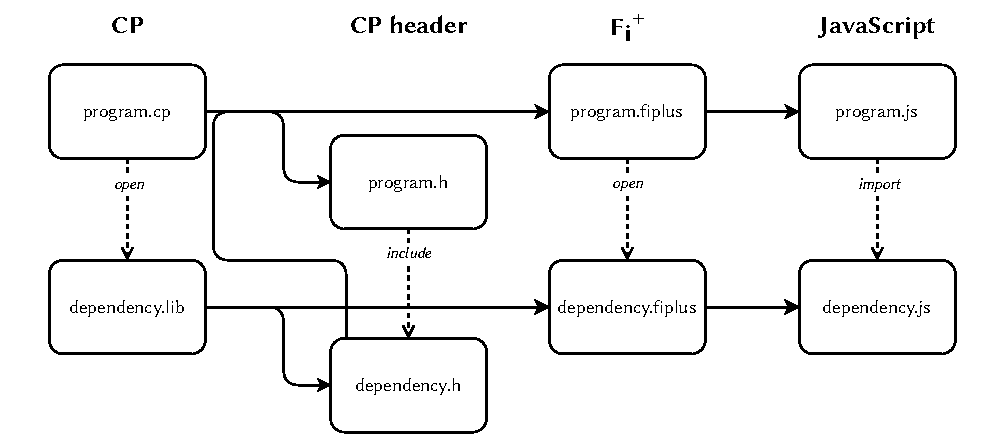
\includegraphics[width=\textwidth]{flowchart.pdf}
\caption{A flowchart of separate compilation in CP.} \label{fig:flowchart}
\end{figure}

\begin{figure}
\begin{subfigure}[t]{.5\textwidth}
\begin{lstlisting}
-- example.cp
open strings;
type Rcd = { m: String; n: String };
mkA = trait [this: Rcd] => {
  m = "foobar";
  n = toUpperCase this.m;
};
\end{lstlisting}
\end{subfigure}%
\begin{subfigure}[t]{.5\textwidth}
\begin{lstlisting}[morekeywords={include,term}]
-- example.cp.h
include "strings.lib.h";
type Rcd = { m: String; n: String };
term mkA :
  Trait<{ m: String }&{ n: String }
     => { m: String }&{ n: String }>;
\end{lstlisting}
\end{subfigure}
\caption{A CP file and its corresponding header file.} \label{fig:header}
\end{figure}

The flowchart in \autoref{fig:flowchart} gives an overview of the compilation
process from CP all the way down to JavaScript, which is almost a textbook
example of separate compilation. Like most programming languages, the
compilation unit of CP is a file. One can refer to another file using
\lstinline{open} directives in CP, which compile to JavaScript module
\lstinline[language=TypeScript]{import} statements. To provide sufficient type
information for modular type checking, a CP file compiles to a JavaScript file
as well as a CP header file. CP header files are similar to \lstinline{.mli}
files in OCaml and consist of type definitions, type signatures for terms, and
references to other header files. See \autoref{fig:header} for a slightly
simplified example. Normally, header files are automatically generated by the CP
compiler, but users can also edit them to hide some definitions that are
supposed to be private. The compilation only depends on the file to be compiled
and the headers files of its dependencies. As a result, compiling a file does
not require recursively compiling its dependencies, and its dependents do not
need recompilation as long as its header file is not changed (though its
implementations may have changed).

Between CP and JavaScript, there is a core calculus
\fiplus~\citep{bi2019distributive,fan2022direct}. Since our implementation of CP
is based on the elaboration semantics formalized by
\citet{zhang2021compositional}, CP language constructs are first desugared into
\fiplus terms, and then these \fiplus terms are compiled into JavaScript code.
Both sets of elaboration rules are syntax-directed and compositional, and the
elaboration contexts only include type information from header files in our
implementation. That is why CP code can be separately compiled with the help of
header files.
